\centerline{\bf \Huge Теорема Кадзи}

В этом листочке рассмотрим некое обобщение теоремы Птолемея и его применения.

\section{Доказательство основного утверждения}

\textit{Вспомогательная лемма.}
Две окружности $S_1$ и $S_2$, радиусы которых равны $r_1$ и $r_2$, касаются окружности радиуса $r$ в точках $A$ и $B$. Рассмотрим общую касательную к $S_1$ и $S_2$, причем внешнюю, если касания одинаковые и внутреннюю, если разные. Тогда длина этой касательной равна $AB \cdot \dfrac{\sqrt{\left(r \pm r_1\right)\left(r \pm r_2\right)}}{r}$ где знак «+» ставится в случае внешнего касания, а знак «---» - внутреннего. (Можно считать, что $r>r_1, r>r_2$.)

\begin{proof}
    Есть три различные ситуации, которые на самом то деле почти одинаковы --- одна касается внутренним образом, другая внешним, обе касаются внешним образом и обе касаются внутренним образом. Разберем сперва первый случай. 

\begin{tcolorbox}[
    enhanced,
    breakable,
    colback=gray!10,
    colframe=blue!70!black,
    colbacktitle=blue!85!black,
    coltitle=white,
    fonttitle=\bfseries,
    title=Задача о радикальной оси вписанных в сегмент окружностей.,
    boxrule=0.8pt,
    arc=2mm
]

\textit{В окружности $\Omega$ проведена хорда $B C$. В один из отсекаемых ею сегментов вписаны две окружности $\omega_1$ и $\omega_2$. Докажите, что середина дуги $B C$ окружности $\Omega$, не касающейся окружностей $\omega_1$ и $\omega_2$, лежит на радикальной оси окружностей $\omega_1$ и $\omega_2$.}

\end{tcolorbox}

\begin{proof}
    Докажем, что степень середины $X$ дуги $B C$ окружности $\Omega$ относительно любой окружности $\omega$, вписанной в сегмент, отсекаемой хордой $B C$, постоянная и равна $B X^2$. Действительно, рассмотрим произвольную окружность $\omega$, касающуюся окружности $\Omega$ в точке $A$ и хорды $B C$ в точке $K$. По лемме Архимеда точки $A, K$ и $X$ лежат на одной прямой, так что степень точки $X$ относительно окружности $\omega$ равна $Q K \cdot X A$. С другой стороны, треугольники $X A B$ и $X B K$ подобны по двум углам (угол $\angle X$ у них общий, а углы $\angle X A B$ и $\angle X B K$ смотрят на равные дуги и потому тоже равны). Отсюда следует, что $X B: X K=X A: X B$ и $X K \cdot X A=X B^2$, что и требовалось доказать.
\end{proof}

Вернёмся к изначальной задаче. Используя только что доказанный факт, понимаем что четырёхугольник $AA'B'B$ вписанный. А значит $\vartriangle XAB \sim \vartriangle XB'A'$. Запишем два соотношения

$$
\dfrac{A'B'}{AB} = \dfrac{XA'}{XB} \qquad \qquad \dfrac{A'B'}{AB} = \dfrac{XB'}{XA}
$$

Перемножим, возьмем корень и получим, что $A'B' = AB \cdot \sqrt{\dfrac{XA'}{XA}\cdot\dfrac{XB'}{XB}}$.


\begin{figure}[h]
    \centering
    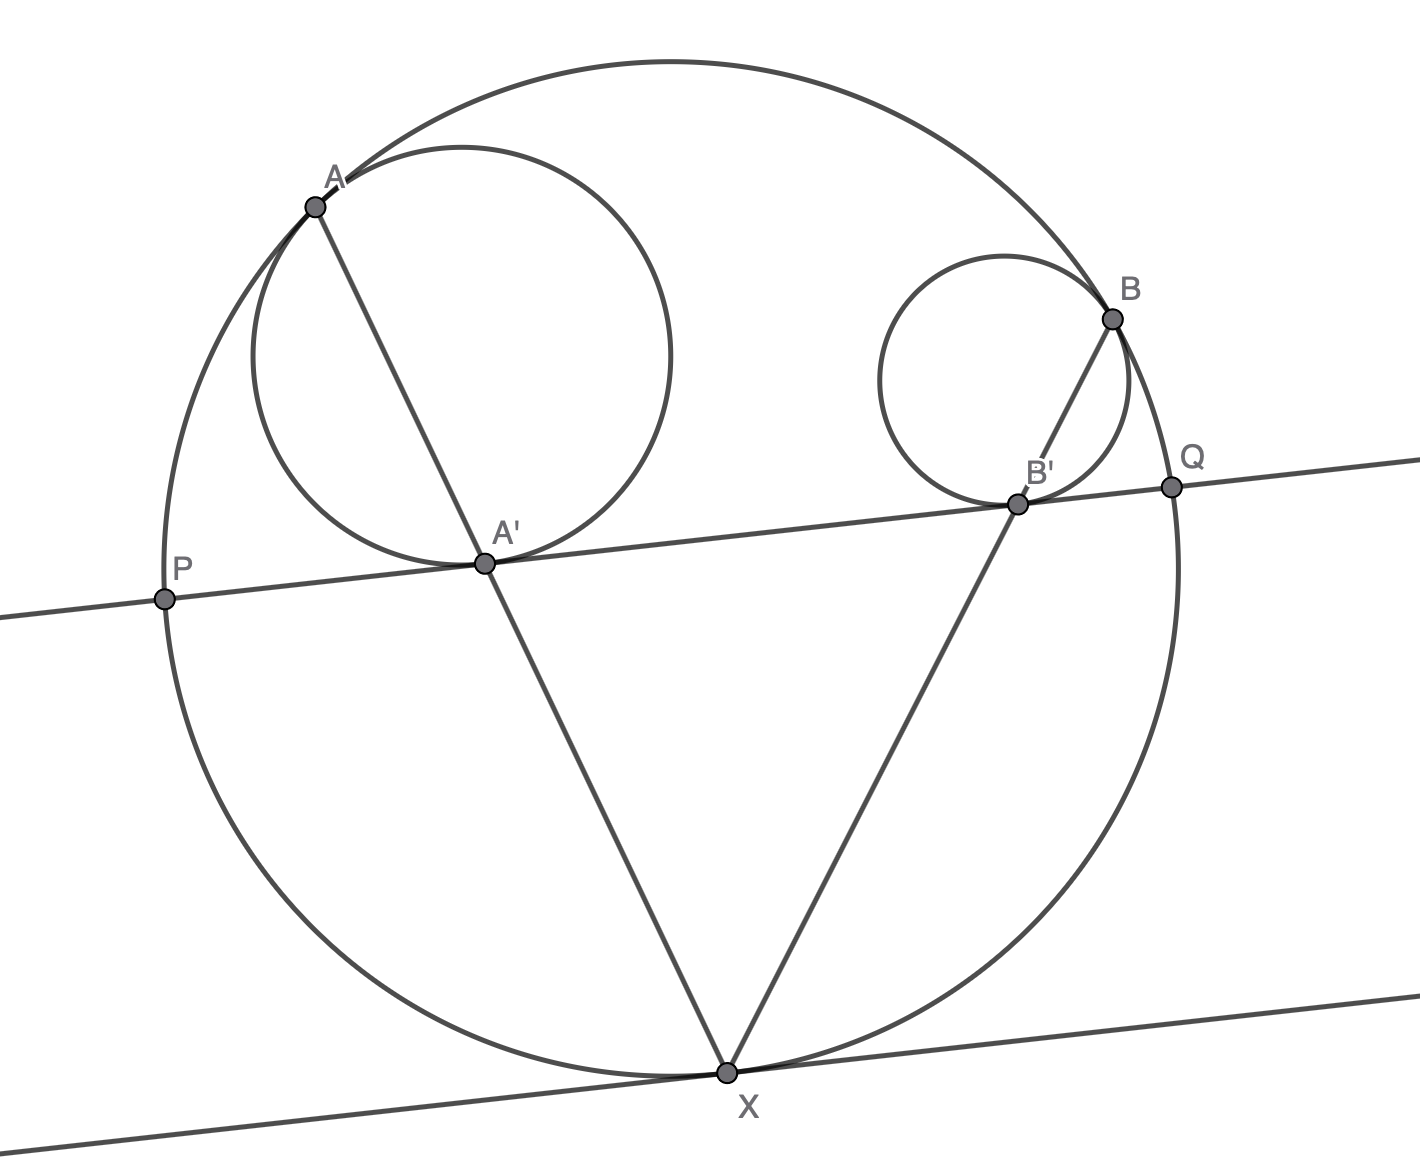
\includegraphics[width=0.5\linewidth]{Теория//Теорема Кэзи/casey_lemma_1.png}
    \caption{Обе окружности касаются внутренним образом}
    \label{fig:placeholder}
\end{figure}

Так как окружность $S_1$ и окружность радиуса $r$ гомотетичны с коэффициентом $\dfrac{r_1}{r}$ имеем, что $\dfrac{AA'}{XA} = \dfrac{r_1}{r}$. Тогда $\dfrac{XA'}{XA} = \dfrac{XA - AA'}{XA} = 1 - \dfrac{r_1}{r} = \dfrac{r - r_1}{r}$. Аналогично $\dfrac{XB'}{XB} = \dfrac{r-r_2}{r}$. Подставляем и получаем то что нужно.

\begin{figure}[h]
    \centering
    \begin{minipage}{0.48\textwidth}
        \centering
        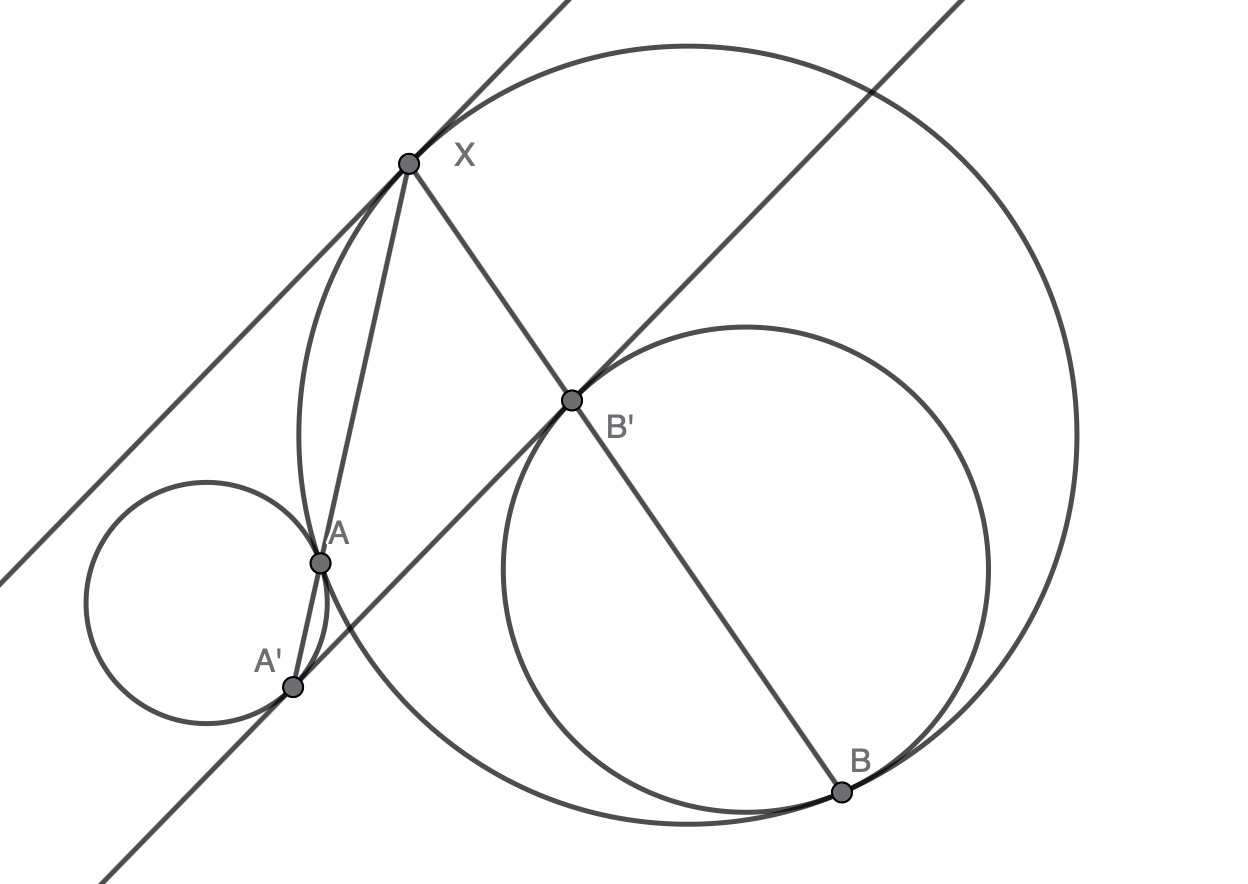
\includegraphics[width=\linewidth]{Теория//Теорема Кэзи/casey_lemma_2.png}
        \caption{Окружности с разными видами касания}
        \label{fig:casey2}
    \end{minipage}
    \hfill
    \begin{minipage}{0.48\textwidth}
        \centering
        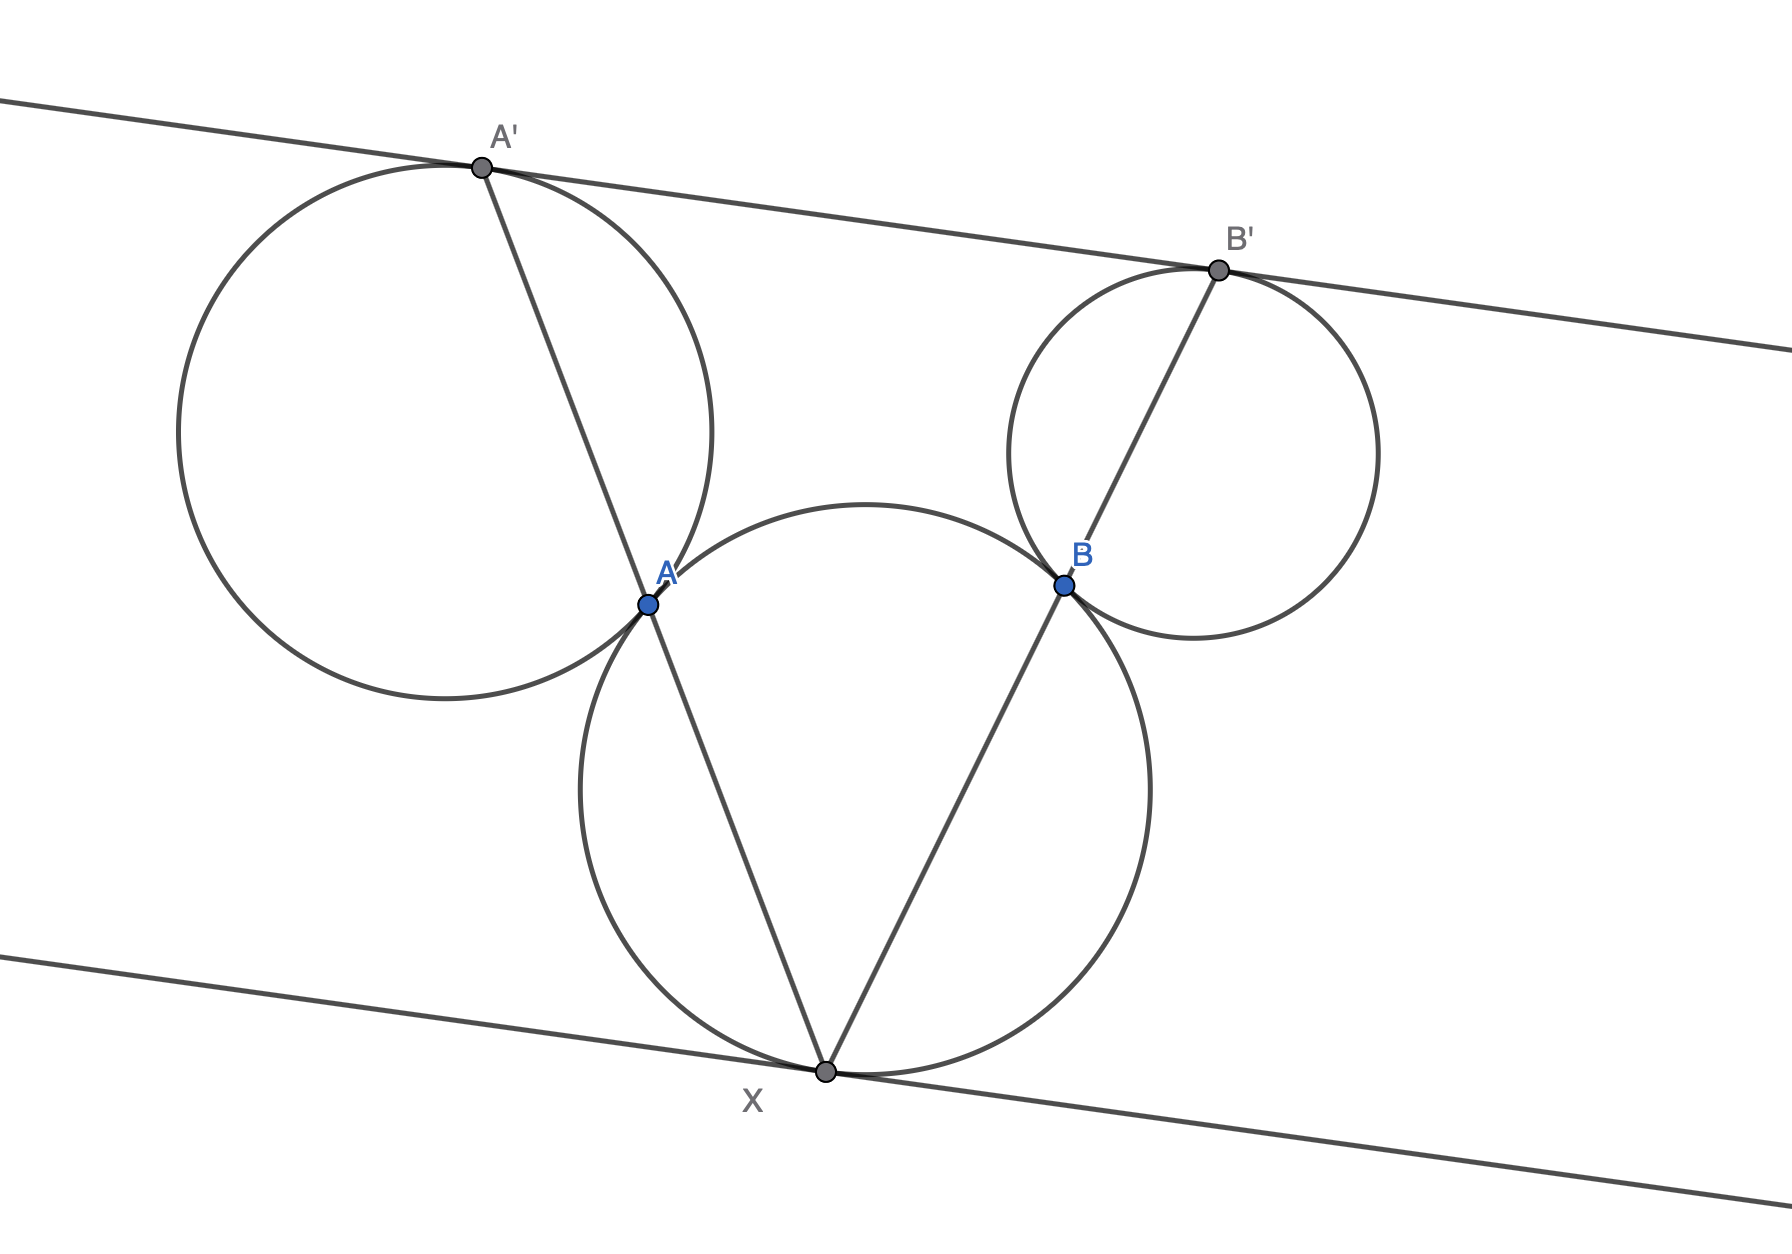
\includegraphics[width=\linewidth]{Теория//Теорема Кэзи/casey_lemma_3.png}
        \caption{Обе окружности касаются внешним образом}
        \label{fig:casey3}
    \end{minipage}
\end{figure}


Вторая и третья ситуация отличаются лишь в последнем шаге, всё остальное работает точно так же. Если, например, $S_1$ касается внешним образом, то соотношение $\dfrac{XA'}{XA}$ переписывается следующим образом:

$$
\dfrac{XA'}{XA} = \dfrac{XA + AA'}{XA} = 1+ \dfrac{r_1}{r} = \dfrac{r+r_1}{r}
$$

Отсюда и появляются эти странные условия про плюсы и минусы. Вспомогательная лемма полностью доказана.

\end{proof}


\begin{tcolorbox}[
    enhanced,
    breakable,
    colback=gray!10,
    colframe=blue!70!black,
    colbacktitle=blue!85!black,
    coltitle=white,
    fonttitle=\bfseries,
    title= Теорема Кэзи,
    boxrule=0.8pt,
    arc=2mm
]

Дан четырехугольник $A B C D$, вписанный в окружность $S$. Рассмотрим окружности $S_A, S_B, S_C, S_D$, касающиеся $S$ в точках $A, B, C, D$ соответственно. Обозначим через $t_{A B}$ длину общей касательной к $S_A$ и $S_B$, причем касательная внешняя, если $S_A$ и $S_B$ касаются $S$ одинаковым образом и внутренняя, если разным. Аналогичным образом определяются величины $t_{A C}, t_{A D}, t_{B C}, t_{B D}, t_{C D}$. Тогда $t_{A B} t_{C D}+t_{B C} t_{A D}=t_{A C} t_{B D}$.

\end{tcolorbox}

\begin{proof}
    Теперь доказательство теоремы Кэзи не составит никакого труда. Используя доказанную лемму получаем:
\[
\begin{gathered}
t_{AB}t_{CD} = AB\cdot CD \cdot \dfrac{\sqrt{(r\pm r_a)(r\pm r_b)(r\pm r_c)(r\pm r_d)}}{r^2}\\
t_{BC}t_{AD} = BC\cdot AD \cdot \dfrac{\sqrt{(r\pm r_a)(r\pm r_b)(r\pm r_c)(r\pm r_d)}}{r^2}\\
t_{AC}t_{BD} = AC\cdot BD \cdot \dfrac{\sqrt{(r\pm r_a)(r\pm r_b)(r\pm r_c)(r\pm r_d)}}{r^2}
\end{gathered}
\]

\begin{figure}[h]
    \centering
    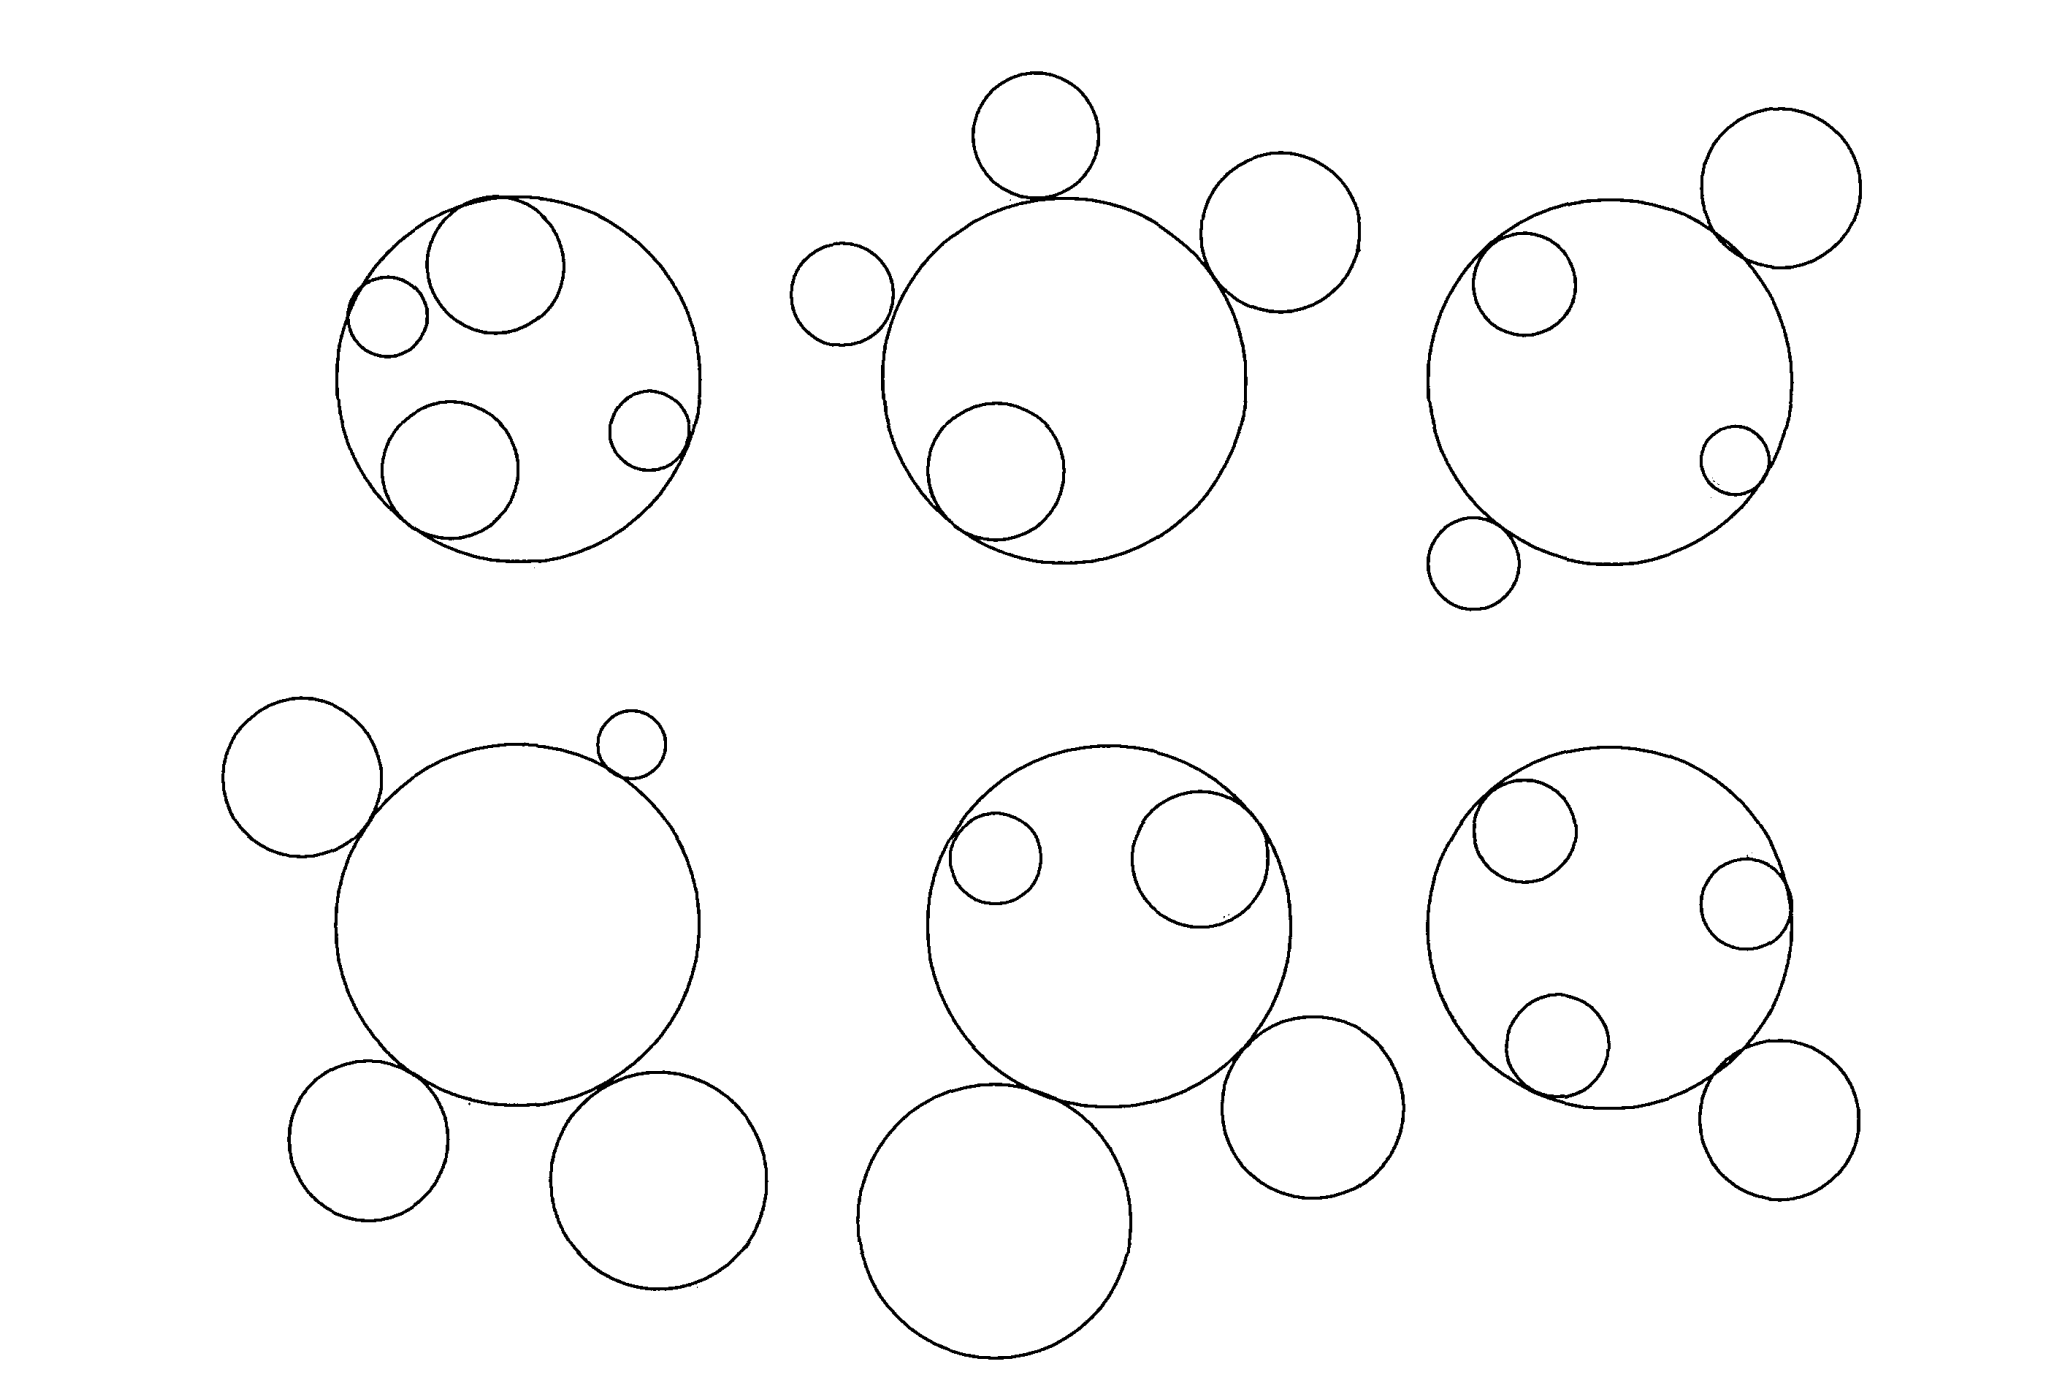
\includegraphics[width=0.5\linewidth]{Теория//Теорема Кэзи/6 случаев касания.png}
    \caption{Шесть различных случаев касания в теореме Кэзи}
    \label{fig:placeholder}
\end{figure}

Тогда равенство $t_{A B} t_{C D}+t_{B C} t_{A D}=t_{A C} t_{B D}$ после сокращения на общий множитель превращается в формулировку теоремы Птолемея. Теорема Кэзи доказана.

\end{proof}

\section{Примеры применения и слабая теорема Кэзи}


Прежде чем приступать к решению задач сформулируем так называемую <<слабую теорему Кэзи>>.

\begin{tcolorbox}[
    enhanced,
    breakable,
    colback=gray!10,
    colframe=blue!70!black,
    colbacktitle=blue!85!black,
    coltitle=white,
    fonttitle=\bfseries,
    title= Слабая версия теоремы Кэзи,
    boxrule=0.8pt,
    arc=2mm
]

Предположим, что на плоскости даны окружность $\omega$ три точки $A, B, C$ вне неё, не лежащие на одной прямой. Обозначим длины отрезков касательных из точек $A, B, C$ к окружности $\omega$ через $t_a, t_b, t_c$ соответственно. Тогда окружность $(ABC)$ касается окружности $\omega$ в том и в только в том случае, если для некоторой расстановки знаков «+» и «-» выполнено соотношение

$$
\pm t_a \cdot B C \pm t_b \cdot C A \pm t_c \cdot A B=0 .
$$

\end{tcolorbox}

В формулировке теоремы Кэзи никто не запрещал нам брать окружности нулевого радиуса. В слабой версии это и было проделано --- точки $A,B,C$ это просто окружности нулевого радиуса. Сила слабой теоремы Кэзи в том, что у нас появляется довольно крутой критерий касания двух окружностей через счёт отрезков, ранее мы это умели делать в основном через счёт уголков.

\begin{tcolorbox}[
    enhanced,
    breakable,
    colback=gray!10,
    colframe=green!70!black,
    colbacktitle=green!85!black,
    coltitle=black,
    fonttitle=\bfseries,
    title= Пример 1,
    boxrule=0.8pt,
    arc=2mm
]

Дан равнобедренный треугольник $A B C$, в котором $A B=A C$. Окружность $\omega$ касается $B C$ и дуги $B C$ описанной окружности треугольника $A B C$. Касательная из точки $A$ к $\omega$ касается $\omega$ в точке $P$. Найдите ГМТ всех таких точек $P$ при изменении окружности $\omega$.

\end{tcolorbox}


\begin{proof}
    Определим точки $A,B,C$ как окружности нулевого радиуса и применим слабую теорему Кэзи к четверке $(A,B,C,\omega)$. Получим, что $AB\cdot CX + AC\cdot BX = BC\cdot AP$, где $X$ точка касания $BC$ и $\omega$. Так как $AB=AC$ получаем, что $AB\cdot(CX + BX) = BX\cdot AP$ или же $AB = AP$. То есть точка $P$ лежит на дуге окружности с центром в точке $A$ и радиусом равным боковой стороне треугольника $ABC$.

Вот \href{https://www.geogebra.org/calculator/egjqxhrb}{тут} можно посмотреть на визуализацию

\begin{figure}[h]
    \centering
    
\includegraphics[width=0.5\linewidth]{Теория//Теорема Кэзи/example_1.png}
    \caption{ГМТ точки P это дуга}
    \label{fig:placeholder}
\end{figure}

\end{proof}


\begin{tcolorbox}[
    enhanced,
    breakable,
    colback=gray!10,
    colframe=green!70!black,
    colbacktitle=green!85!black,
    coltitle=black,
    fonttitle=\bfseries,
    title= Пример 2,
    boxrule=0.8pt,
    arc=2mm
]

\textit{(Теорема Фейербаха)}.
Окружность девяти точек касается вписанной и всех трех вневписанных окружностей треугольника.
\end{tcolorbox}

\begin{proof}
    Сперва покажем, что окружность Эйлера касается вписанной окружности, которую назовём $\omega$. Пусть $BC = a, AC = b, AB = c$. Нам достаточно проверить критерий касания по слабой теореме Кэзи для четверки $(A_1, B_1, C_1, \omega)$. 

    $t_{A_1}\omega = A_1A_2$ --- касательная из $A_1$ к $\omega$. Аналогично определим $t_{B_1}\omega = B_1B_2$  и $t_{C_1}\omega = C_1C_2$. Известно, что $BA_2 = BC_2 = \dfrac{a-b+c}{2}$, $CA_2 = CB_2 = \dfrac{a+b-c}{2}$ и $AB_2 = AC_2 = \dfrac{-a+b+c}{2}$. Теперь мы готовы к финальным вычислениям.

    $t_{A_1}\cdot B_1C_1 - t_{B_1}\cdot A_1C_1 + t_{C_1}\cdot A_1B_1 = \left(\dfrac{c}{2}-\dfrac{c+a-b}{2}\right) \cdot \dfrac{c}{2}+\left(\dfrac{a}{2}-\dfrac{a+b-c}{2}\right) \cdot \dfrac{a}{2}+\left(\dfrac{b}{2}-\dfrac{b+c-a}{2}\right) \cdot \dfrac{b}{2} = (b-a) \cdot c+(c-b) \cdot a+(a-c) \cdot b = 0$. Что и требовалось доказать.

    Вторую часть теоремы предлагается доказать самостоятельно.

    \begin{figure}[h]
        \centering
        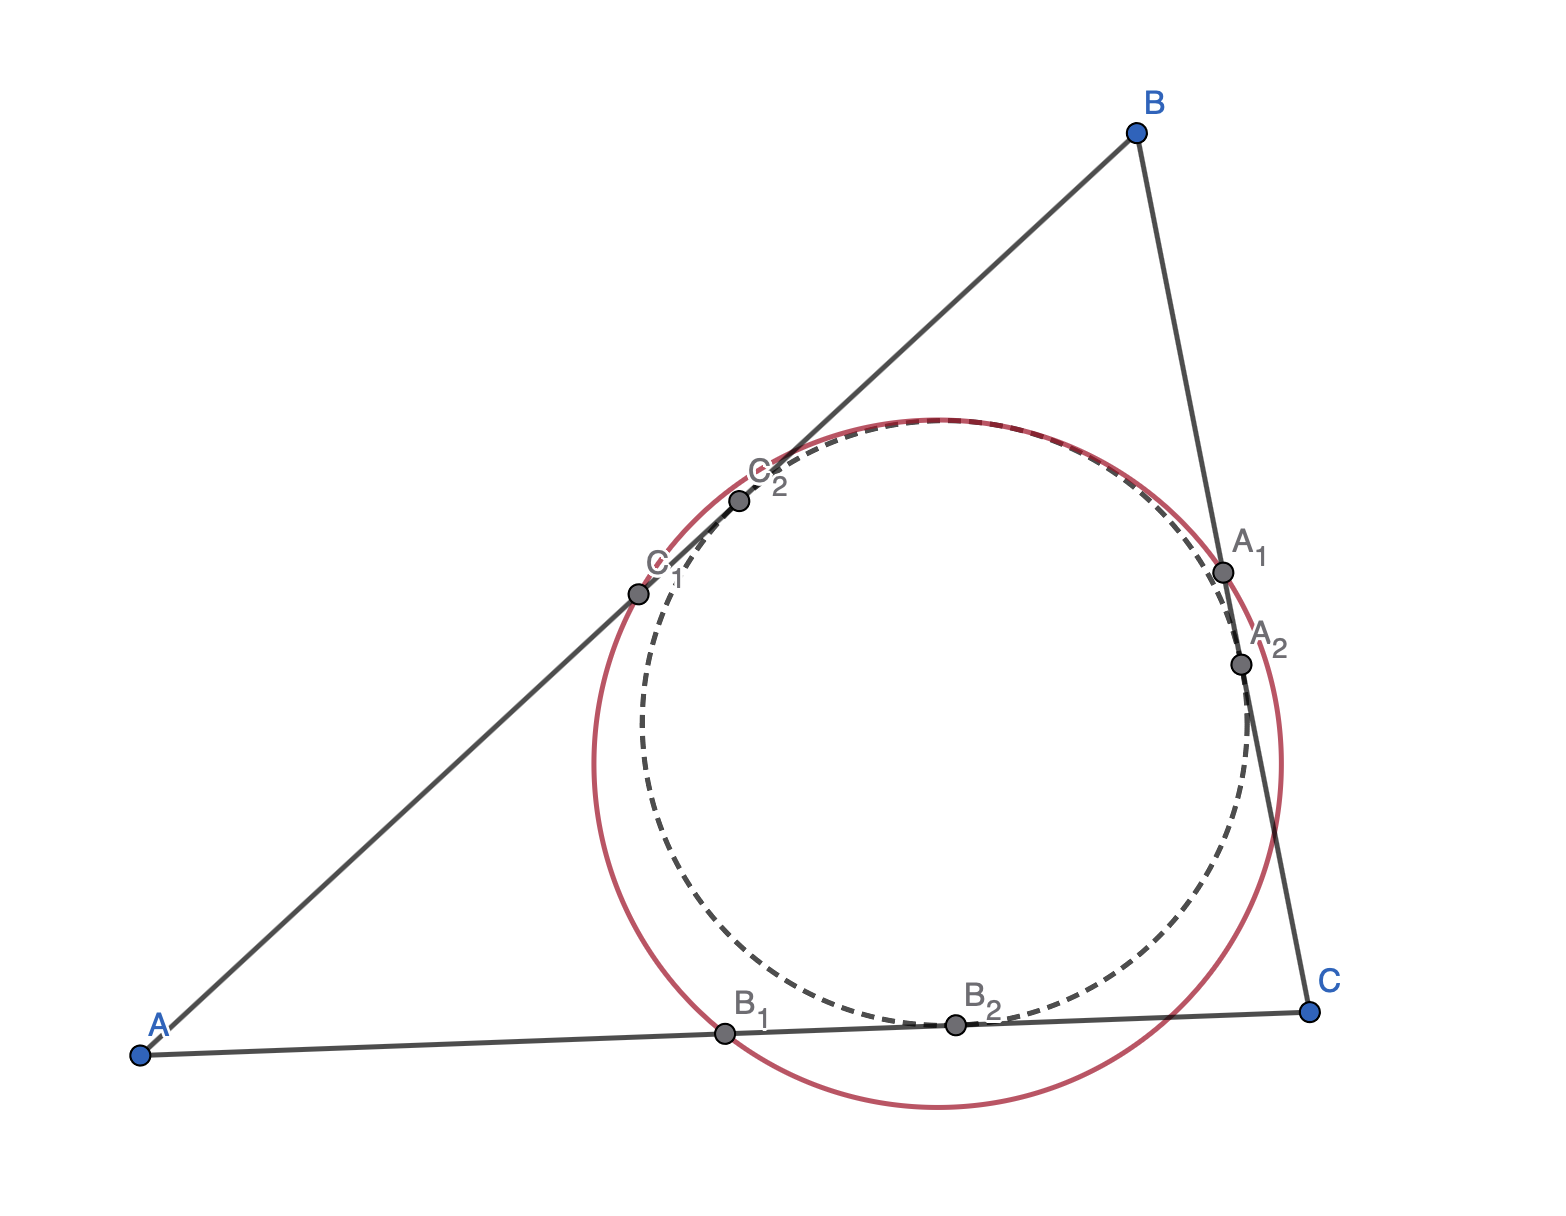
\includegraphics[width=0.5\linewidth]{Теория//Теорема Кэзи/Feuerbach_incirc.png}
        \caption{Красным цветом окружность Эйлера, пунктиром --- вписанная}
        \label{fig:placeholder}
    \end{figure}
    
\end{proof}

\begin{tcolorbox}[
    enhanced,
    breakable,
    colback=gray!10,
    colframe=green!70!black,
    colbacktitle=green!85!black,
    coltitle=black,
    fonttitle=\bfseries,
    title= Пример 3. Версия на английском,
    boxrule=0.8pt,
    arc=2mm
]

$\bigl[\textbf{ \href{https://artofproblemsolving.com/downloads/printable_post_collections/3943?srsltid=AfmBOooNkI5vOXvq4RX2I7bobkxnFolYh1hqmCT5O4jGM7gKoQIVdAgE}{IMO Shortlist 1992, Problem 7}}\bigr]$
Two circles $\Omega_1$ and $\Omega_2$ are externally tangent to each other at a point $I$, and both of these circles are tangent to a third circle $\Omega$ which encloses the two circles $\Omega_1$ and $\Omega_2$.
The common tangent to the two circles $\Omega_1$ and $\Omega_2$ at the point $I$ meets the circle $\Omega$ at a point $A$. One common tangent to the circles $\Omega_1$ and $\Omega_2$ which doesn't pass through $I$ meets the circle $\Omega$ at the points $B$ and $C$ such that the points $A$ and $I$ lie on the same side of the line $B C$. Prove that the point $I$ is the incenter of triangle $A B C$.


\end{tcolorbox}


\begin{tcolorbox}[
    enhanced,
    breakable,
    colback=gray!10,
    colframe=green!70!black,
    colbacktitle=green!85!black,
    coltitle=black,
    fonttitle=\bfseries,
    title= Пример 3. Версия на русском,
    boxrule=0.8pt,
    arc=2mm
]

Две окружности $\Omega_1$ и $\Omega_2$ касаются друг друга внешним образом в точке $I$, и обе эти окружности касаются третьей окружности $\Omega$, которая содержит внутри себя окружности $\Omega_1$ и $\Omega_2$. Общая касательная к окружностям $\Omega_1$ и $\Omega_2$ в точке $I$ пересекает окружность $\Omega$ в точке $A$. Одна из общих касательных к окружностям $\Omega_1$ и $\Omega_2$, не проходящая через $I$, пересекает окружность $\Omega$ в точках $B$ и $C$ так, что точки $A$ и $I$ лежат по одну сторону от прямой $B C$. Докажите, что точка $I$ является центром вписанной окружности треугольника $A B C$.

\end{tcolorbox}

\newpage

\hspace{3mm}

\begin{proof}
    Обозначим через $X\Omega_k$ длину касательной из точки $X$ к окружности $\Omega_k$. Точку будем считать вырожденной окружностью радиуса $0$.

Пусть
\[
AI \cap BC = D,\qquad BI \cap AC = E,\qquad CI \cap AB = F.
\]

Применим теорему Кэзи к четырём окружностям $(B), \Omega_1, (A), \Omega_2$, которые все касаются окружности $\Omega$. Получаем
\[
B\Omega_1 \cdot A\Omega_2 + B\Omega_2 \cdot A\Omega_1
=
AB \cdot \Omega_1\Omega_2.
\]
Так как $AI$ является общей касательной к $\Omega_1$ и $\Omega_2$ в точке $I$, то
\[
A\Omega_1 = A\Omega_2 = AI.
\]
Следовательно,
\[
AI(B\Omega_1+B\Omega_2)=AB\cdot \Omega_1\Omega_2. \tag{1}
\]

Аналогично, применяя теорему Кэзи к четырём окружностям $(C), \Omega_1, (A), \Omega_2$, получаем
\[
C\Omega_1 \cdot A\Omega_2 + C\Omega_2 \cdot A\Omega_1
=
AC \cdot \Omega_1\Omega_2,
\]
откуда
\[
AI(C\Omega_1+C\Omega_2)=AC\cdot \Omega_1\Omega_2. \tag{2}
\]

Складывая $(1)$ и $(2)$, имеем
\[
AI(B\Omega_1+B\Omega_2+C\Omega_1+C\Omega_2)
=
(AB+AC)\Omega_1\Omega_2.
\]
Пусть прямая $BC$ касается окружностей $\Omega_1$ и $\Omega_2$ в точках $T_1$ и $T_2$ соответственно. Тогда
\[
B\Omega_1+C\Omega_1=BT_1+CT_1=BC,\qquad
B\Omega_2+C\Omega_2=BT_2+CT_2=BC.
\]
Значит,
\[
B\Omega_1+B\Omega_2+C\Omega_1+C\Omega_2=2BC.
\]
Поэтому
\[
2BC\cdot AI=(AB+AC)\Omega_1\Omega_2. \tag{3}
\]

\newpage

\hspace{3mm}

Теперь выразим $\Omega_1\Omega_2$. Точка $D$ лежит на пересечении двух общих касательных к $\Omega_1$ и $\Omega_2$: прямых $AI$ и $BC$. Поэтому длины касательных из точки $D$ к каждой из окружностей равны:
\[
DI=DT_1,\qquad DI=DT_2.
\]
Так как точки $T_1$ и $T_2$ лежат по разные стороны от $D$, получаем
\[
\Omega_1\Omega_2=T_1T_2=DT_1+DT_2=2DI.
\]
Подставляя это в $(3)$, получаем
\[
2BC\cdot AI=2(AB+AC)DI,
\]
то есть
\[
\dfrac{AI}{ID}=\dfrac{AB+AC}{BC}. \tag{4}
\]

Аналогично, применяя тот же аргумент к сторонам $AC$ и $AB$, получаем
\[
\dfrac{BI}{IE}=\dfrac{BA+BC}{AC}, \tag{5}
\]
\[
\dfrac{CI}{IF}=\dfrac{CA+CB}{AB}. \tag{6}
\]

Из $(4)$ следует
\[
\dfrac{AI}{AD}
=
\dfrac{AB+AC}{AB+AC+BC}.
\]
Аналогично из $(5)$ и $(6)$ получаем
\[
\dfrac{BI}{BE}
=
\dfrac{BA+BC}{AB+AC+BC},
\qquad
\dfrac{CI}{CF}
=
\dfrac{CA+CB}{AB+AC+BC}.
\]

Положим
\[
a=BC,\qquad b=CA,\qquad c=AB.
\]
Тогда
\[
\dfrac{AI}{AD}=\dfrac{b+c}{a+b+c},\qquad
\dfrac{BI}{BE}=\dfrac{c+a}{a+b+c},\qquad
\dfrac{CI}{CF}=\dfrac{a+b}{a+b+c}.
\]
Эти равенства означают, что барицентрические координаты точки $I$ равны
\[
(a:b:c).
\]

\newpage

\hspace{3mm}

Но точка с барицентрическими координатами $(a:b:c)$ является инцентром треугольника $ABC$. Действительно,
\[
[IBC]:[ICA]:[IAB]=a:b:c,
\]
а значит расстояния от $I$ до сторон $BC, CA, AB$ равны. Следовательно, точка $I$ равноудалена от всех сторон треугольника $ABC$, то есть является центром его вписанной окружности.

Значит, $I$ --- инцентр треугольника $ABC$.
\end{proof}
\section{Когда применять теорему Кэзи?}

Я думаю это плюс минус стало понятно после приведенных примеров. Теорему Кэзи стоит применять когда есть надобность в доказательстве касания двух окружностей и в особенности тогда, когда много отрезков касания. Зачастую помогает именно слабая версия, где какие-то точки можно считать окружностями нулевого радиуса и причем понятно, что их необязательно 3, может быть и 2 точки с двумя полноценными окружностями.